\def\year{2017}\relax
%File: formatting-instruction.tex
\documentclass[letterpaper]{article} %DO NOT CHANGE THIS
\usepackage{aaai18}  %Required
\usepackage{times}  %Required
\usepackage{helvet}  %Required
\usepackage{courier}  %Required
\usepackage{url}  %Required
\usepackage{graphicx}  %Required
\frenchspacing  %Required
\setlength{\pdfpagewidth}{8.5in}  %Required
\setlength{\pdfpageheight}{11in}  %Required
%PDF Info Is Required:
  \pdfinfo{}
\setcounter{secnumdepth}{0}

\usepackage{amsmath}
\usepackage{amssymb}
\usepackage{amsthm}
\usepackage{multirow}
\usepackage{tikz}
\usepackage{comment}

\usepackage{graphicx}
\usepackage{caption}
\usepackage{subcaption}
\usepackage{listings}
\usepackage{multicol}
\usepackage{arydshln}
\usetikzlibrary{calc,backgrounds,positioning,fit}


\newcommand{\tup}[1]{{\langle #1 \rangle}}

\newcommand{\pre}{\mathsf{pre}}     % precondition
\newcommand{\del}{\mathsf{del}}     % effect
\newcommand{\add}{\mathsf{add}}     % effect
\newcommand{\eff}{\mathsf{eff}}     % effect
\newcommand{\cond}{\mathsf{cond}}   % conditional effect
\newcommand{\true}{\mathsf{true}}   % true
\newcommand{\false}{\mathsf{false}} % false
\newcommand{\PE}{\mathrm{PE}}     % precondition
\newcommand{\strips}{\textsc{Strips}}     % precondition



\newtheorem{theorem}{Theorem}
\newtheorem{lemma}[theorem]{Lemma}
\newtheorem{definition}[theorem]{Definition}


\begin{document}

\title{Learning \strips\ action models with classical planning}
\author{\#39}


% Commented for blind submission
\author{Diego Aineto\and Sergio Jim\'enez\and Eva Onaindia\\
{\small Departamento de Sistemas Inform\'aticos y Computaci\'on}\\
{\small Universitat Polit\`ecnica de Val\`encia.}\\
{\small Camino de Vera s/n. 46022 Valencia, Spain}\\
{\small \{dieaigar,serjice,onaindia\}@dsic.upv.es}}

\maketitle
\begin{abstract}
This paper presents a novel approach for learning \strips\ action models from examples that compiles this inductive learning task into classical planning. Interestingly, the compilation approach is flexible to different amounts of available input knowledge; the learning examples can range from a set of plans (with their corresponding initial and final states) to just a set of initial and final states (no intermediate action or state is given). What is more, the compilation accepts partially specified action models and can be used to validate whether the observation of a plan execution follows a given \strips\ action model, even if this model is not fully specified.
\end{abstract}


\section{Introduction}
Besides {\em plan synthesis}~\cite{ghallab2004automated}, planning action models are also useful for {\em plan/goal recognition}~\cite{ramirez2012plan}. At both planning tasks, an automated planner is required to reason about action models that correctly and completely capture the possible world transitions~\cite{geffner:book:2013}. Unfortunately, building planning action models is complex, even for planning experts, and this knowledge acquisition task is a bottleneck that limits the potential of AI planning~\cite{kambhampati:modellite:AAAI2007}.

On the other hand, Machine Learning (ML) has shown to be able to compute a wide range of different kinds of models from examples~\cite{michalski2013machine}. The application of inductive ML to the learning of \strips\ action models, the vanilla action model for planning~\cite{fikes1971strips}, is not straightforward though:
\begin{itemize}
\item The {\em input} to ML algorithms (the learning/training data) usually are finite vectors encoding the value of fixed features in a given set of objects. The input for learning planning action models are observations of plan executions (where each plan possibly has a different length).
\item The {\em output} of ML algorithms usually is a scalar value (an integer, in the case of {\em classification} tasks, or a real value, in the case of {\em regression} tasks). When learning \strips\ action models the output is, for each action, the sets of preconditions, negative and positive effects, that define the possible state transitions.
\end{itemize}

Learning \strips\ action models is a well-studied problem with sophisticated algorithms, like {\sc ARMS}~\cite{yang2007learning}, {\sc SLAF}~\cite{amir:alearning:JAIR08} or {\sc LOCM}~\cite{cresswell2013acquiring} that do not require full knowledge of the intermediate states traversed by the example plans. Motivated by recent advances on the synthesis of different kinds of generative models with classical planning~\cite{bonet2009automatic,segovia2016hierarchical,segovia2017generating}, this paper introduces an innovative approach for learning \strips\ action models that can be defined as a classical planning compilation. The compilation approach is appealing by itself because opens the door to the bootstrapping of planning action models but also because:
\begin{enumerate}
\item Is flexible to different amounts of available input knowledge. The learning examples can range from a set of plans (with their corresponding initial and final states) to just a set of initial and final states where no intermediate state  or action is observed.
\item Accepts previous knowledge about the structure of the actions in the form of partially specified action models. In the extreme, the compilation can validate whether an observed plan execution is valid for a given \strips\ action model, even if this model is not fully specified.
\end{enumerate}

The second section of the paper formalizes the classical planning model, its extension to {\em conditional effects} (a requirement of the proposed compilation) and the \strips\ action model (the output of the addressed learning task). The third section formalizes the learning of \strips\ action models with regard to different amounts of available input knowledge. The fourth and fifth sections describe our approach for addressing the formalized learning tasks. Finally, the last sections report the data collected in a empirical evaluation, discuss the strengths and weaknesses of our approach and propose several opportunities for future research.


\section{Background}
This section defines the planning models used on this work and the output of the learning tasks addressed in the paper.

\subsection{Classical planning}
We use $F$ to denote the set of {\em fluents} (propositional variables) describing a state. A {\em literal} $l$ is a valuation of a fluent $f\in F$, i.e. either~$l=f$ or $l=\neg f$. A set of literals $L$ represents a partial assignment of values to fluents (WLOG we assume that $L$ does not assign conflicting values to any fluent). We use $\mathcal{L}(F)$ to denote the set of all literal sets on $F$, i.e.~all partial assignments of values to fluents.

A {\em state} $s$ is a full assignment of values to fluents, i.e. $|s|=|F|$, so the size of the state space is $2^{|F|}$. Explicitly including negative literals $\neg f$ in states simplifies subsequent definitions but often, we will abuse notation by defining a state $s$ only in terms of the fluents that are true in $s$, as is common in \strips\ planning.

A {\em classical planning frame} is a tuple $\Phi=\tup{F,A}$, where $F$ is a set of fluents and $A$ is a set of actions. Each action $a\in A$ comprises three sets of literals:
\begin{itemize}
\item $\pre(a)\subseteq\mathcal{L}(F)$, called {\em preconditions}, the literals that must hold for the action $a\in A$ to be applicable.
\item $\eff^+(a)\subseteq\mathcal{L}(F)$, called {\em positive effects}, that defines the fluents set to true by the application of the action $a\in A$.
\item $\eff^-(a)\subseteq\mathcal{L}(F)$, called {\em negative effects}, that defines the fluents set to false by the action application.
\end{itemize}
We say that an action $a\in A$ is {\em applicable} in a state $s$ iff $\pre(a)\subseteq s$. The result of applying $a$ in $s$ is the {\em successor state} $\theta(s,a)=\{s\setminus\eff^-(a))\cup\eff^+(a)\}$.

A {\em classical planning problem} is a tuple $P=\tup{F,A,I,G}$, where $I$ is an initial state and $G\subseteq\mathcal{L}(F)$ is a goal condition. A {\em plan} for $P$ is an action sequence $\pi=\tup{a_1, \ldots, a_n}$ that induces a state sequence $\tup{s_0, s_1, \ldots, s_n}$ such that $s_0=I$ and, for each {\small $1\leq i\leq n$}, $a_i$ is applicable in $s_{i-1}$ and generates the successor state $s_i=\theta(s_{i-1},a_i)$. We denote with $|\pi|$ the {\em plan length}. A plan $\pi$ {\em solves} $P$ iff $G\subseteq s_n$, i.e.~if the goal condition is satisfied at the last state reached after following the application of $\pi$ in $I$.


\subsection{Classical planning with conditional effects}
Our approach for learning \strips\ action models is compiling this leaning task into a classical planning task with conditional effects. Conditional effects allow us to compactly define actions whose effects depend on the current state. Supporting conditional effects is now a requirement of the IPC~\cite{vallati:IPC:AIM2015} and many classical planners cope with conditional effects without compiling them away.

An action $a\in A$ has now a set of {\em preconditions} $\pre(a)\in\mathcal{L}(F)$ and a set of {\em conditional effects} $\cond(a)$. Each conditional effect $C\rhd E\in\cond(a)$ is composed of two sets of literals $C\in\mathcal{L}(F)$, the {\em condition}, and $E\in\mathcal{L}(F)$, the {\em effect}.

An action $a\in A$ is {\em applicable} in a state $s$ if and only if $\pre(a)\subseteq s$, and the resulting set of {\em triggered effects} are the effects whose conditions hold in $s$:
\[
triggered(s,a)=\bigcup_{C\rhd E\in\cond(a),C\subseteq s} E,
\]

The result of applying an action $a$ in a state $s$ is the {\em successor} state $\theta(s,a)=\{s\setminus\eff_c^-(s,a))\cup\eff_c^+(s,a)\}$ where $\eff_c^-(s,a)\subseteq triggered(s,a)$ and $\eff_c^+(s,a)\subseteq triggered(s,a)$ are the triggered {\em negative} and {\em positive} effects, respectively.


\subsection{\strips\ action schemes and {\em variable name} objects}
This work addresses the learning of PDDL action schemes that follow the \strips\ requirement~\cite{mcdermott1998pddl,fox2003pddl2}. Figure~\ref{fig:stack} shows the schema, coded in PDDL, for the {\em stack} action from a four-operator {\em blocksworld}~\cite{slaney2001blocks}.

\begin{figure}
\begin{footnotesize}
\begin{verbatim}
(:action stack
  :parameters (?v1 ?v2 - object)
  :precondition (and (holding ?v1) (clear ?v2))
  :effect (and (not (holding ?v1))
               (not (clear ?v2))
               (handempty) (clear ?v1)
               (on ?v1 ?v2)))
\end{verbatim}
\end{footnotesize}
 \caption{\small \strips\ operator schema coding, in PDDL, the {\em stack} action from the {\em blocksworld}.}
\label{fig:stack}
\end{figure}

To formalize the output of the learning task, we assume that fluents $F$ are instantiated from a set of {\em predicates} $\Psi$, as in PDDL. Each predicate $p\in\Psi$ has an argument list of arity $ar(p)$. Given a set of {\em objects} $\Omega$, the set of fluents $F$ is induced by assigning objects in $\Omega$ to the arguments of predicates in $\Psi$, i.e.~$F=\{p(\omega):p\in\Psi,\omega\in\Omega^{ar(p)}\}$ s.t. $\Omega^k$ is the $k$-th Cartesian power of $\Omega$.

Let $\Omega_v=\{v_i\}_{i=1}^{\operatorname*{max}_{a\in A} ar(a)}$ be a new set of objects $\Omega\cap\Omega_v=\emptyset$, denoted as {\em variable names}, and that is bound by the maximum arity of an action in a given planning frame. For instance, in a three-block blocksworld $\Omega=\{block_1, block_2, block_3\}$ while $\Omega_v=\{v_1, v_2\}$ because the operators with the maximum arity, {\small\tt stack} and {\small\tt unstack}, have two parameters each.

Let us also define $F_v$, a new set of fluents $F\cap F_v=\emptyset$, that results from instantiating $\Psi$ using only the objects in $\Omega_v$ and that defines the elements that can appear in an action schema. For instance, in the blocksworld, $F_v$={\small\tt\{handempty, holding($v_1$), holding($v_2$), clear($v_1$), clear($v_2$), ontable($v_1$), ontable($v_2$), on($v_1,v_1$), on($v_1,v_2$), on($v_2,v_1$), on($v_2,v_2$)\}}.

Finally, we assume that actions $a\in A$ are instantiated from \strips\ operator schemes $\xi=\tup{head(\xi),pre(\xi),add(\xi),del(\xi)}$ where:
\begin{itemize}
\item $head(\xi)=\tup{name(\xi),pars(\xi)}$, is the operator {\em header} defined by its name and corresponding {\em variable names}, $pars(\xi)=\{v_i\}_{i=1}^{ar(\xi)}$. For instance, the headers for a four-operator blocksworld are: {\small\tt pickup($v_1$), putdown($v_1$), stack($v_1,v_2$)} and {\small\tt unstack($v_1,v_2$)}.
\item The preconditions $pre(\xi)\subseteq F_v$, the negative effects $del(\xi)\subseteq F_v$, and the positive effects $add(\xi)\subseteq F_v$ such that, $del(\xi)\subseteq pre(\xi)$, $del(\xi)\cap add(\xi)=\emptyset$ and $pre(\xi)\cap add(\xi)=\emptyset$.
\end{itemize}


\section{Learning \strips\ action models}
Learning \strips\ action models from fully available input knowledge, i.e. from plans where the {\em pre-} and {\em post-states} of every action in a plan are available, is straightforward. When any intermediate state is available, \strips\ operator schemes are derived lifting the literals that change between the pre and post-state of the corresponding action executions. Preconditions are derived lifting the minimal set of literals that appears in all the pre-states of the corresponding actions.

This section formalizes more challenging learning tasks, where less input knowledge is available:

\subsubsection{Learning from (initial, final) state pairs.} This learning task corresponds to observing an agent acting in the world but watching only the results of its plan executions. No information about the actions in the plans is given. This learning task is formalized as $\Lambda=\tup{\Psi,\Sigma}$:
\begin{itemize}
\item $\Psi$ is the set of predicates that define the abstract state space of a given planning domain.
\item $\Sigma=\{\sigma_1,\ldots,\sigma_{\tau}\}$ is a set of $(initial, final)$ state pairs, that we call {\em labels}. Each label $\sigma_t=(s_0^t,s_{n}^t)$, {\tt\small $1\leq t\leq \tau$}, comprises the {\em final} state $s_{n}^t$ resulting from executing an unknown plan $\pi_t$ starting from the {\em initial} state $s_0^t$.
\end{itemize}

\subsubsection{Learning from labeled plans.}
Here we augment the input knowledge with the actions executed by the observed agent and define the learning task $\Lambda'=\tup{\Psi,\Sigma,\Pi}$:

\begin{itemize}
\item $\Pi=\{\pi_1,\ldots,\pi_{\tau}\}$ is a given set of example plans where each plan $\pi_t=\tup{a_1^t, \ldots, a_n^t}$, {\small $1\leq t\leq \tau$}, is an action sequence that induces the corresponding state sequence $\tup{s_0^t, s_1^t, \ldots, s_n^t}$ such that, for each {\small $1\leq i\leq n$}, $a_i^t$ is applicable in $s_{i-1}^t$ and generates $s_i^t=\theta(s_{i-1}^t,a_i^t)$.
\end{itemize}

Figure~\ref{fig:lexample} shows an example of a learning task $\Lambda'$ in the blocksworld. This learning task has a single learning example, $\Pi=\{\pi_1\}$ and $\Sigma=\{\sigma_1\}$, that corresponds to observing the execution of an eight-action plan $(|\pi_1|=8)$ for inverting a four-block tower.

\subsubsection{Learning from partially specified action models.}
We may not require to start learning from scratch so we augment the learning input with partially specified operator schemes. This leaning task is defined as $\Lambda''=\tup{\Psi,\Sigma,\Pi,\Xi_0}$:
\begin{itemize}
\item $\Xi_0$ is a partially specified action model in which some preconditions and effects are a priori known.
\end{itemize}

A solution to $\Lambda$ is a set of operator schema $\Xi$ that is compliant just with the predicates in $\Psi$, and the given set of initial and final states $\Sigma$. In this learning scenario, a solution must not only determine a possible \strips\ action model but also the plans $\pi_t$, {\tt\small $1\leq t\leq \tau$} that explain the given labels $\Sigma$ using the learned \strips\ model. A solution to $\Lambda'$ is a set of \strips\ operator schema $\Xi$ (one schema $\xi=\tup{head(\xi),pre(\xi),add(\xi),del(\xi)}$ for each action with a different name in the example plans $\Pi$) compliant with the predicates in $\Psi$, the example plans $\Pi$, and their corresponding labels $\Sigma$.  Finally a solution to $\Lambda''$ is a set of \strips\ operator schema $\Xi$ compliant as well with the provided partially specified action model $\Xi_0$.

\begin{figure}
{\tt ;;; Predicates in $\Psi$}
\begin{footnotesize}
\begin{verbatim}
(handempty) (holding ?o  - object)
(clear ?o - object) (ontable ?o - object)
(on ?o1 - object ?o2 - object)
\end{verbatim}
\end{footnotesize}

\vspace{0.2cm}

\begin{subfigure}{.25\textwidth}
{\tt ;;; Plan $\pi_1$}
\begin{footnotesize}
\begin{verbatim}
0: (unstack A B)
1: (putdown A)
2: (unstack B C)
3: (stack B A)
4: (unstack C D)
5: (stack C B)
6: (pickup D)
7: (stack D C)
\end{verbatim}
\end{footnotesize}
\end{subfigure}%
\begin{subfigure}{.6\textwidth}
{\tt ;;; Label $\sigma_1=(s_0^1,s_{n}^1)$}
\begin{lstlisting}[mathescape]
\end{lstlisting}
\vspace{0.1cm}
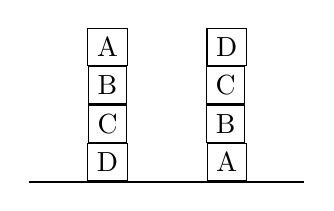
\begin{tikzpicture}[node distance = 0mm, block/.style args = {#1,#2}{fill=#1,text width=#2,shape=square}]
\node (initD) [draw]{D};
\node (initC) [draw, above=of initD.north]{C};
\node (initB) [draw, above=of initC.north]{B};
\node (initA) [draw, above=of initB.north]{A};
\draw[thick] (-1,-0.25) -- (2.5,-0.25);

\node (goalA) [draw, right=10mm of initD]{A};
\node (goalB) [draw, right=10mm of initC]{B};
\node (goalC) [draw, right=10mm of initB]{C};
\node (goalD) [draw, right=10mm of initA]{D};
\end{tikzpicture}
\vspace{0.6cm}
\end{subfigure}%
 \caption{\small Example of a task for learning a \strips\ action model in the blocksworld from a single labeled plan.}
\label{fig:lexample}
\end{figure}


\section{Learning \strips\ action models with planning}
Our approach for addressing a learning task $\Lambda$, $\Lambda'$ or $\Lambda''$, is compiling it into a classical planning task with conditional effects. The intuition behind the compilation is that a solution to the resulting classical planning task is a sequence of actions that:
\begin{enumerate}
\item Programs the \strips\ action model $\Xi$. A solution plan has a {\em prefix} that, for each $\xi\in\Xi$, determines the fluents from $F_v$ that belong to its $pre(\xi)$, $del(\xi)$ and $add(\xi)$ sets.
\item Validates the programmed \strips\ action model $\Xi$ in the given input knowledge (the labels $\Sigma$, and $\Pi$ and/or $\Xi_0$ if available). For every label $\sigma_t\in \Sigma$, a solution plan has a postfix that produces a final state $s_{n}^t$ starting from the corresponding initial state $s_0^t$ using the programmed action model $\Xi$. We call this process the validation of the programmed \strips\ action model $\Xi$, at the learning example {\small $1\leq t\leq \tau$}. %If information about the corresponding plan $\pi_t\in \Pi$ is available, then it is also used in the validation.
\end{enumerate}

To formalize our compilation we first define {\small $1\leq t\leq \tau$} classical planning instances $P_t=\tup{F,\emptyset,I_t,G_t}$ that belong to the same planning frame (i.e. same fluents and actions but differ in the initial state and goals). Fluents $F$ are built instantiating the predicates in $\Psi$ with the objects appearing in the input labels $\Sigma$. Formally $\Omega=\{o|o\in \bigcup_{\small 1\leq t\leq \tau} obj(s_0^t)\}$, where $obj$ is a function that returns the set of objects that appear in a fully specified state. The set of actions, $A=\emptyset$, is empty because the action model is initially unknown. Finally, the initial state $I_t$ is given by the state $s_0^t\in \sigma_t$ while goals $G_t$, are defined by the state $s_n^t\in \sigma_t$.

Now we are ready to formalize the compilations. We start with $\Lambda$, because it requires less input knowledge. Given a learning task $\Lambda=\tup{\Psi,\Sigma}$ the compilation outputs a classical planning task $P_{\Lambda}=\tup{F_{\Lambda},A_{\Lambda},I_{\Lambda},G_{\Lambda}}$:
\begin{itemize}
\item $F_{\Lambda}$ extends $F$ with:
\begin{itemize}
\item Fluents representing the programmed action model $pre_f(\xi)$, $del_f(\xi)$ and $add_f(\xi)$, for every $f\in F_v$ and $\xi \in \Xi$. If a fluent $pre_f(\xi)/del_f(\xi)/add_f(\xi)$ holds, it means that $f$ is a precondition/negative effect/positive effect in the \strips\ operator schema $\xi\in \Xi$. For instance, the preconditions of the $stack$ schema (Figure~\ref{fig:stack}) are represented by fluents {\small\tt pre\_holding\_stack\_$v_1$} and {\small\tt pre\_clear\_stack\_$v_2$}.
\item A fluent $mode_{prog}$ indicating whether the operator schemes are being programmed or validated (already programmed) and fluents $\{test_t\}_{1\leq t\leq \tau}$, indicating the example where the action model is being validated.
\end{itemize}
\item $I_{\Lambda}$ contains the fluents from $F$ that encode $s_0^1$ (the initial state of the first label), every $pre_f(\xi)\in F_{\Lambda}$ and $mode_{prog}$ set to true. Our compilation assumes that initially any operator schema is programmed with every possible precondition, no negative effect and no positive effect.
\item $G_{\Lambda}=\bigcup_{1\leq t\leq \tau}\{test_t\}$, indicates that the programmed action model is validated in all the learning examples.
\item $A_{\Lambda}$ contains actions of three kinds:
\begin{enumerate}
\item Actions for {\em programming} an operator schema $\xi\in\Xi$:
\begin{itemize}
\item Actions for {\bf removing} a {\em precondition} $f\in F_v$ from the action schema $\xi\in\Xi$.

\begin{small}
\begin{align*}
\hspace*{7pt}\pre(\mathsf{programPre_{f,\xi}})=&\{\neg del_{f}(\xi),\neg add_{f}(\xi),\\
& mode_{prog}, pre_{f}(\xi)\},\\
\cond(\mathsf{programPre_{f,\xi}})=&\{\emptyset\}\rhd\{\neg pre_{f}(\xi)\}.
\end{align*}
\end{small}

\item Actions for {\bf adding} a {\em negative} or {\em positive} effect $f\in F_v$ to the action schema $\xi\in\Xi$.

\begin{small}
\begin{align*}
\hspace*{7pt}\pre(\mathsf{programEff_{f,\xi}})=&\{\neg del_{f}(\xi),\neg add_{f}(\xi),\\
& mode_{prog}\},\\
\cond(\mathsf{programEff_{f,\xi}})=&\{pre_{f}(\xi)\}\rhd\{del_{f}(\xi)\},\\
&\{\neg pre_{f}(\xi)\}\rhd\{add_{f}(\xi)\}.
\end{align*}
\end{small}
\end{itemize}

\item Actions for {\em applying} an already programmed operator schema $\xi\in\Xi$ bound with the objects $\omega\subseteq\Omega^{ar(\xi)}$. We assume operators headers are known so the binding of the operator schema is done implicitly by order of appearance of the action parameters, i.e. variables $pars(\xi)$ are bound to the objects in $\omega$ appearing at the same position. Figure~\ref{fig:compilation} shows the PDDL encoding of the action for applying a programmed operator $stack$.
\begin{small}
\begin{align*}
\hspace*{7pt}\pre(\mathsf{apply_{\xi,\omega}})=&\{pre_{f}(\xi)\implies p(\omega)\}_{\forall p\in\Psi,f=p(pars(\xi))},\\
\cond(\mathsf{apply_{\xi,\omega}})=&\{del_{f}(\xi)\}\rhd\{\neg p(\omega)\}_{\forall p\in\Psi,f=p(pars(\xi))},\\
&\{add_{f}(\xi)\}\rhd\{p(\omega)\}_{\forall p\in\Psi,f=p(pars(\xi))},\\
&\{mode_{prog}\}\rhd\{\neg mode_{prog}\}.
\end{align*}
\end{small}

\item Actions for {\em validating} the learning example {\tt\small $1\leq t\leq \tau$}.
\begin{small}
\begin{align*}
\hspace*{7pt}\pre(\mathsf{validate_{t}})=&G_t\cup\{test_j\}_{j\in 1\leq j<t}\\
&\cup\{\neg test_j\}_{j\in t\leq j\leq \tau}\cup \{\neg mode_{prog}\},\\
\cond(\mathsf{validate_{t}})=&\{\emptyset\}\rhd\{test_t\}.
\end{align*}
\end{small}
\end{enumerate}
\end{itemize}

\begin{lemma}
Any classical plan $\pi$ that solves $P_{\Lambda}$ induces an action model $\Xi$ that solves the learning task $\Lambda$.
\end{lemma}

\begin{proof}[Proof sketch]
\begin{small}
The compilation forces that once the preconditions of an operator schema $\xi \in \Xi$ are programmed, they cannot be altered. The same happens with the positive and negative effects that define an operator schema $\xi \in \Xi$ (besides they can only be programmed after preconditions are programmed). Once operator schemes are programmed they can only be applied because of the $mode_{prog}$ fluent. To solve $P_{\Lambda}$, goals $\{test_t\}$, {\small $1\leq t\leq \tau$} can only be achieved: executing an applicable sequence of programmed operator schemes that reaches the final state $s_n^t$, defined in $\sigma_t$, starting from $s_0^t$. If this is achieved for all the input examples {\small $1\leq t\leq \tau$}, it means that the programmed action model $\Xi$ is compliant with the provided input knowledge and hence, it is a solution to $\Lambda$.
\end{small}
\end{proof}

The compilation is {\em complete} in the sense that it does not discard any possible \strips\ action model.


\begin{figure}
\begin{scriptsize}
\begin{verbatim}
(:action apply_stack
  :parameters (?o1 - object ?o2 - object)
  :precondition
   (and (or (not (pre_on_stack_v1_v1)) (on ?o1 ?o1))
        (or (not (pre_on_stack_v1_v2)) (on ?o1 ?o2))
        (or (not (pre_on_stack_v2_v1)) (on ?o2 ?o1))
        (or (not (pre_on_stack_v2_v2)) (on ?o2 ?o2))
        (or (not (pre_ontable_stack_v1)) (ontable ?o1))
        (or (not (pre_ontable_stack_v2)) (ontable ?o2))
        (or (not (pre_clear_stack_v1)) (clear ?o1))
        (or (not (pre_clear_stack_v2)) (clear ?o2))
        (or (not (pre_holding_stack_v1)) (holding ?o1))
        (or (not (pre_holding_stack_v2)) (holding ?o2))
        (or (not (pre_handempty_stack)) (handempty)))
  :effect
   (and (when (del_on_stack_v1_v1) (not (on ?o1 ?o1)))
        (when (del_on_stack_v1_v2) (not (on ?o1 ?o2)))
        (when (del_on_stack_v2_v1) (not (on ?o2 ?o1)))
        (when (del_on_stack_v2_v2) (not (on ?o2 ?o2)))
        (when (del_ontable_stack_v1) (not (ontable ?o1)))
        (when (del_ontable_stack_v2) (not (ontable ?o2)))
        (when (del_clear_stack_v1) (not (clear ?o1)))
        (when (del_clear_stack_v2) (not (clear ?o2)))
        (when (del_holding_stack_v1) (not (holding ?o1)))
        (when (del_holding_stack_v2) (not (holding ?o2)))
        (when (del_handempty_stack) (not (handempty)))
        (when (add_on_stack_v1_v1) (on ?o1 ?o1))
        (when (add_on_stack_v1_v2) (on ?o1 ?o2))
        (when (add_on_stack_v2_v1) (on ?o2 ?o1))
        (when (add_on_stack_v2_v2) (on ?o2 ?o2))
        (when (add_ontable_stack_v1) (ontable ?o1))
        (when (add_ontable_stack_v2) (ontable ?o2))
        (when (add_clear_stack_v1) (clear ?o1))
        (when (add_clear_stack_v2) (clear ?o2))
        (when (add_holding_stack_v1) (holding ?o1))
        (when (add_holding_stack_v2) (holding ?o2))
        (when (add_handempty_stack) (handempty))
        (when (modeProg) (not (modeProg)))))
\end{verbatim}
\end{scriptsize}
 \caption{\small Action for applying an already programmed schema $stack$ as encoded in PDDL (implications coded as disjunctions).}
\label{fig:compilation}
\end{figure}

\section{Constraining the learning hypothesis space with additional input knowledge}
\label{sec:Constraining}
Here we show that further input knowledge can be used to constrain the space of possible action models and make the learning of \strips\ action models more practicable.

\subsection{Labeled plans}
We extend the compilation to consider labeled plans. Given a learning task $\Lambda'=\tup{\Psi,\Sigma,\Pi}$, the compilation outputs a classical planning task $P_{\Lambda'}=\tup{F_{\Lambda'},A_{\Lambda'},I_{\Lambda'},G_{\Lambda'}}$ that extends $P_{\Lambda}$ as follows:
\begin{itemize}
\item $F_{\Lambda'}$ extends $F_{\Lambda}$ with $F_{\Pi}=\{plan(name(\xi),\Omega^{ar(\xi)},j)\}$, the fluents to code the steps of the plans in $\Pi$, where $F_{\pi_t}\subseteq F_{\Pi}$ encodes $\pi_t\in \Pi$. Fluents $at_j$ and $next_{j,j_2}$, {\small $1\leq j<j2\leq n$}, are also added to represent the current plan step and to iterate through the steps of a plan.
\item $I_{\Lambda'}$ extends $I_{\Lambda}$ with fluents $F_{\pi_1}$ plus fluents $at_1$ and $\{next_{j,j_2}\}$, {\small $1\leq j<j2\leq n$}, for indicating the plan step where the action model is validated. Goals are $G_{\Lambda'}=G_{\Lambda}=\bigcup_{1\leq t\leq \tau}\{test_t\}$, as in the original compilation.
\item With respect to $A_{\Lambda'}$.
\begin{enumerate}
\item The actions for {\em programming} the preconditions/effects of a given operator schema $\xi\in\Xi$ are the same.
\item The actions for {\em applying} an already programmed operator have an extra precondition $f\in F_{\Pi}$, that encodes the current plan step, and extra conditional effects $\{at_{j}\}\rhd\{\neg at_{j},at_{j+1}\}_{\forall j\in [1,n]}$ for advancing to the next plan step. This mechanism forces that these actions are only applied as in the example plans.
\item The actions for {\em validating} the current learning example have an extra precondition, $at_{|\pi_t|}$, to indicate that the current plan $\pi_t$ was fully executed and extra conditional effects to unload plan $\pi_{t}$ and load the next plan $\pi_{t+1}$:
\begin{small}
\begin{align*}
&\{\emptyset\}\rhd\{\neg at_{|\pi_t|},at_1\}, \{f\}\rhd\{\neg f\}_{f\in F_{\pi_t}}, \{\emptyset\}\rhd\{f\}_{f\in F_{\pi_t+1}}.
\end{align*}
\end{small}
\end{enumerate}
\end{itemize}

\subsection{Partially specified action models}
Known preconditions and effects are encoded as fluents $pre_f(\xi)$, $del_f(\xi)$ and $add_f(\xi)$ set to true at the initial state $I_{\Lambda'}$. The corresponding programming actions, $\mathsf{programPre_{f,\xi}}$ and $\mathsf{programEff_{f,\xi}}$, become unnecessary and are removed from $A_{\Lambda'}$ making the classical planning task $P_{\Lambda'}$ easier to be solved.

To illustrate this, the classical plan of Figure~\ref{fig:plan} is a solution to a learning task $\Lambda''=\tup{\Psi,\Sigma,\Pi,\Xi_0}$ for getting the blocksworld action model where operator schemes for {\tt\small pickup}, {\tt\small putdown} and {\tt\small unstack} are specified in $\Xi_0$. This plan programs and validates the operator schema {\tt\small stack} from the blocksworld, using the plan $\pi_1$ and label $\sigma_1$ shown in Figure~\ref{fig:lexample}. Plan steps $[0,8]$ are the actions for programming the preconditions of the {\tt\small stack} operator, steps $[9,13]$ are the actions for programming the operator effects and steps $[14,22]$ are the actions for validating the programmed operators following the plan $\pi_1$ shown in the Figure~\ref{fig:lexample}.

In the extreme, when a fully specified \strips\ action model $\Xi$ is given in $\Xi_0$, the compilation validates whether an observed plan follows the given model. In this case, if a solution plan is found to $P_{\Lambda'}$, it means that the given \strips\ action model is {\em valid} for the given examples. If $P_{\Lambda'}$ is unsolvable it means that the given \strips\ action model is invalid since it is not compliant with all the given examples. Tools for plan validation like VAL~\cite{howey2004val} could also be used at this point.

\begin{figure}
{\tt\small
     {\bf 00} : (program\_pre\_clear\_stack\_v1)\\
     01 : (program\_pre\_handempty\_stack)\\
     02 : (program\_pre\_holding\_stack\_v2)\\
     03 : (program\_pre\_on\_stack\_v1\_v1)\\
     04 : (program\_pre\_on\_stack\_v1\_v2)\\
     05 : (program\_pre\_on\_stack\_v2\_v1)\\
     06 : (program\_pre\_on\_stack\_v2\_v2)\\
     07 : (program\_pre\_ontable\_stack\_v1)\\
     08 : (program\_pre\_ontable\_stack\_v2)\\
     {\bf 09} : (program\_eff\_clear\_stack\_v1)\\
    10 : (program\_eff\_clear\_stack\_v2)\\
    11 : (program\_eff\_handempty\_stack)\\
    12 : (program\_eff\_holding\_stack\_v1)\\
    13 : (program\_eff\_on\_stack\_v1\_v2)\\
    {\bf 14} : (apply\_unstack a b i1 i2)\\
    15 : (apply\_putdown a i2 i3)\\
    16 : (apply\_unstack b c i3 i4)\\
    17 : (apply\_stack b a i4 i5)\\
    18 : (apply\_unstack c d i5 i6)\\
    19 : (apply\_stack c b i6 i7)\\
    20 : (apply\_pickup d i7 i8)\\
    21 : (apply\_stack d c i8 i9)\\
    {\bf 22} : (validate\_1)
}
 \caption{\small Plan for programming and validating the $stack$ schema using plan $\pi_1$ and label $\sigma_1$ (shown in Figure~\ref{fig:lexample}) as well as previously specified operator schemes for $pickup$, $putdown$ and $unstack$.}
\label{fig:plan}
\end{figure}

\subsection{Static predicates}
A {\em static predicate} $p \in \Psi$ is a predicate that does not appear in the effects of any action schema~\cite{fox:TIM:JAIR1998}. Therefore, one can get rid of the mechanism for programming these predicates in the effects of any action schema while keeping the compilation complete. Formally, given a static predicate $p$:
\begin{itemize}
\item Fluents $del_f(\xi)$ and $add_f(\xi)$, such that $f\in F_v$ is an instantiation of the static predicate $p$ in the set of {\em variable objects} $\Omega_v$, can be discarded for every $\xi\in\Xi$.
\item Actions $\mathsf{programEff_{f,\xi}}$ (s.t. $f\in F_v$ is an instantiation of $p$ in $\Omega_v$) can also be discarded for every $\xi\in\Xi$.
\end{itemize}

Static predicates can also constrain the space of possible preconditions by looking at the given set of labels $\Sigma$. One can assume that if a precondition $f\in F_v$ (s.t. $f\in F_v$ is an instantiation of a static predicate in $\Omega_v$) is not compliant with the labels in $\Sigma$ then, fluents $pre_f(\xi)$ and actions $\mathsf{programPre_{f,\xi}}$ can be discarded for every $\xi\in\Xi$. For instance in the {\em zenotravel} domain $pre\_next\_board\_v1\_v1$, $pre\_next\_debark\_v1\_v1$, $pre\_next\_fly\_v1\_v1$, $pre\_next\_zoom\_v1\_v1$, $pre\_next\_refuel\_v1\_v1$ can be discarded (and their corresponding programming actions) because a precondition {\tt\small(next ?v1 ?v1 - flevel)} will never hold at any state in $\Sigma$.

Likewise, static predicates can constrain the space of possible preconditions looking at the given example plans. Fluents $pre_f(\xi)$ and actions $\mathsf{programPre_{f,\xi}}$ are discardable for every $\xi\in\Xi$ if a precondition $f\in F_v$ (s.t. $f\in F_v$ is an instantiation of a static predicate in $\Omega_v$) is not possible according to $\Pi$. Back to the {\em zenotravel} domain, if a example plan $\pi_t\in \Pi$ contains the action {\tt\small (fly plane1 city2 city0 fl3 fl2)} and the corresponding label $\sigma_t\in\Sigma$ contains the static literal {\tt\small (next fl2 fl3)} but does not contain {\tt\small (next fl2 fl2)}, {\tt\small (next fl3 fl3)} or {\tt\small (next fl3 fl2)} the only possible precondition including the static predicate is $pre\_next\_fly\_v5\_v4$.

In the evaluation of our approach we do not assume that the set of static predicates is given but compute a set of {\em potential} static predicates from the input to the learning task.


\begin{table*}
		\resizebox{\textwidth}{!}{%                
		\begin{tabular}{l|l|l|l|l|l|l||l|l||l|l|l|l|l|l||l|l|}
& \multicolumn{8}{|c||}{\bf No Static}& \multicolumn{8}{|c|}{\bf Static}\\\cline{2-17}
& \multicolumn{2}{|c|}{\bf Pre} & \multicolumn{2}{|c|}{\bf Add} & \multicolumn{2}{|c|}{\bf Del} & \multicolumn{2}{|c||}{\bf}& \multicolumn{2}{|c|}{\bf Pre} & \multicolumn{2}{|c|}{\bf Add} & \multicolumn{2}{|c|}{\bf Del} & \multicolumn{2}{|c|}{\bf}\\ 			
			  & \multicolumn{1}{|c|}{\bf P} & \multicolumn{1}{|c|}{\bf R} & \multicolumn{1}{|c|}{\bf P} & \multicolumn{1}{|c|}{\bf R} & \multicolumn{1}{|c|}{\bf P} & \multicolumn{1}{|c|}{\bf R} &  \multicolumn{1}{|c|}{\bf P} & \multicolumn{1}{|c||}{\bf R}& \multicolumn{1}{|c|}{\bf P} & \multicolumn{1}{|c|}{\bf R} & \multicolumn{1}{|c|}{\bf P} & \multicolumn{1}{|c|}{\bf R} & \multicolumn{1}{|c|}{\bf P} & \multicolumn{1}{|c|}{\bf R} &  \multicolumn{1}{|c|}{\bf P} & \multicolumn{1}{|c|}{\bf R} \\
                          \hline
			Blocks & 1.0 & 1.0 & 1.0 & 1.0 & 1.0 & 1.0 & 1.0 & 1.0 & 1.0 & 1.0 & 1.0 & 1.0 & 1.0 & 1.0 & 1.0 & 1.0\\
			Driverlog & 1.0 & 0.36 & 0.75 & 0.86 & 1.0 & 0.71 & 0.92 & 0.64 & 0.9 & 0.64 & 0.56 & 0.71 & 0.86 & 0.86 & 0.78 & 0.73\\
			Ferry & 1.0 & 0.57 & 1.0 & 1.0 & 1.0 & 1.0 & 1.0 & 0.86 & 1.0 & 0.57 & 1.0 & 1.0 & 1.0 & 1.0 & 1.0 & 0.86\\
			Floortile & 0.52 & 0.68 & 0.64 & 0.82 & 0.83 & 0.91 & 0.66 & 0.80 & 0.68 & 0.68 & 0.89 & 0.73 & 1.0 & 0.82 & 0.86 & 0.74\\
			Grid & 0.62 & 0.47 & 0.75 & 0.86 & 0.78 & 1.0 & 0.71 & 0.78 & 0.79 & 0.65 & 1.0 & 0.86 & 0.88 & 1.0 & 0.89 & 0.83 \\
			Gripper & 1.0 & 0.67 & 1.0 & 1.0 & 1.0 & 1.0 & 1.0 & 0.89 & 1.0 & 0.67 & 1.0 & 1.0 & 1.0 & 1.0 & 1.0 & 0.89\\
			Hanoi & 1.0 & 0.50 & 1.0 & 1.0 & 1.0 & 1.0 & 1.0 & 0.83 & 0.75 & 0.75 & 1.0 & 1.0 & 1.0 & 1.0 & 0.92 & 0.92\\
			Miconic & 0.75 & 0.33 & 0.50 & 0.50 & 0.75 & 1.0 & 0.67 & 0.61 & 0.89 & 0.89 & 1.0 & 0.75 & 0.75 & 1.0 & 0.88 & 0.88\\
			Satellite & 0.60 & 0.21 & 1.0 & 1.0 & 1.0 & 0.75 & 0.87 & 0.65 & 0.82 & 0.64 & 1.0 & 1.0 & 1.0 & 0.75 & 0.94 & 0.80\\
			Transport & 1.0 & 0.40 & 1.0 & 1.0 & 1.0 & 0.80 & 1.0 & 0.73 & 1.0 & 0.70 & 0.83 & 1.0 & 1.0 & 0.80 & 0.94 & 0.83\\
			Visitall & 1.0 & 0.50 & 1.0 & 1.0 & 1.0 & 1.0 & 1.0 & 0.83 & 1.0 & 1.0 & 1.0 & 1.0 & 1.0 & 1.0 & 1.0 & 1.0\\
			Zenotravel & 1.0 & 0.36 & 1.0 & 1.0 & 1.0 & 0.71 & 1.0 & 0.69 &1.0 & 0.64 & 0.88 & 1.0 & 1.0 & 0.71 & 0.96 & 0.79\\
			\hline
			\bf  & 0.88 & 0.50 & 0.88 & 0.92 & 0.95 & 0.91 & 0.90 & 0.78 & 0.90 & 0.74 & 0.93 & 0.92 & 0.96 & 0.91 & 0.93 & 0.86\\
		\end{tabular}
	}
\caption{\small {\em Precision} and {\em recall} obtained learning from labeled plans without (left) and with (right) static predicates.}
\label{tab:results_plans}
\end{table*}


\begin{table}
\begin{scriptsize}
	\begin{center}
		\begin{tabular}{l|c|c|c||c|c|c|}
                         & \multicolumn{3}{|c||}{\bf No Static}& \multicolumn{3}{|c|}{\bf Static}\\
			 & Total & Preprocess & Length  & Total & Preprocess &  Length\\
                         \hline
			Blocks & 0.04 & 0.00 & 72  & 0.03 & 0.00 & 72 \\
			Driverlog & 0.14 & 0.09 & 83 & 0.06 & 0.03 & 59 \\
			Ferry & 0.06 & 0.03 & 55 & 0.06 & 0.03 & 55 \\
			Floortile & 2.42 & 1.64 & 168 & 0.67 & 0.57 & 77 \\
			Grid & 4.82 & 4.75 & 88 & 3.39 & 3.35 & 72 \\
			Gripper & 0.03 & 0.01 & 43 & 0.01 & 0.00 & 43 \\
                        Hanoi & 0.12 & 0.06 & 48 & 0.09 & 0.06 & 39 \\
                        Miconic & 0.06 & 0.03 & 57 & 0.04 & 0.00 & 41 \\
			Satellite & 0.20 & 0.14 & 67 & 0.18 & 0.12 & 60 \\
			Transport & 0.59 & 0.53 & 61 & 0.39 & 0.35 & 48 \\
			Visitall & 0.21 & 0.15 & 40 & 0.17 & 0.15 & 36 \\
			Zenotravel & 2.07 & 2.04 & 71 & 1.01 & 1.00 & 55 \\			
		\end{tabular}
	\end{center}
        \end{scriptsize}
	\caption{\small Total planning time, preprocessing time and plan length learning from labeled plans without/with static predicates.}
	\label{tab:time_plans}	
\end{table}




\section{Evaluation}
This section evaluates the performance of our approach for learning \strips\ action models starting from different amounts of available input knowledge.

\subsubsection{Setup.}
The domains used in the evaluation are IPC domains that satisfy the \strips\ requirement~\cite{fox2003pddl2}, taken from the {\sc planning.domains} repository~\cite{muise2016planning}. We only use 5 learning examples for each domain and they are fixed for all the experiments so we can evaluate the impact of the input knowledge in the quality of the learned models. All experiments are run on an Intel Core i5 3.10 GHz x 4 with 4 GB of RAM.

\subsubsection{Reproducibility.}
We make fully available the compilation source code, the evaluation scripts and the used benchmarks at this anonymous repository {\em https://github.com/anonsub/strips-learning} so any experimental data reported in the paper is fully reproducible. 

\subsubsection{Planner.}
The classical planner we use to solve the instances that result from our compilations is {\sc Madagascar}~\cite{rintanen2014madagascar}. We use {\sc Madagascar} because its ability to deal with planning instances populated with dead-ends. In addition, SAT-based planners can apply the actions for programming preconditions in a single planning step (in parallel) because these actions do not interact. Actions for programming action effects can also be applied in a single planning step reducing significantly the planning horizon.

\subsubsection{Metrics.}
The quality of the learned models is quantified with the {\em precision} and {\em recall} metrics. These two metrics are frequently used in {\em pattern recognition}, {\em information retrieval} and {\em binary classification} and are more informative that simply counting the number of errors in the learned model or computing the {\em symmetric difference} between the learned and the reference model~\cite{davis2006relationship}.

Intuitively, precision gives a notion of {\em soundness} while recall gives a notion of the {\em completeness} of the learned models. Formally, $Precision=\frac{tp}{tp+fp}$, where $tp$ is the number of true positives (predicates that correctly appear in the action model) and $fp$ is the number of false positives (predicates appear in the learned action model that should not appear). Recall is formally defined as $Recall=\frac{tp}{tp+fn}$ where $fn$ is the number of false negatives (predicates that should appear in the learned action model but are missing).

\subsection{Learning from labeled plans}
We start evaluating our approach at $\Lambda'=\tup{\Psi,\Sigma,\Pi}$ learning tasks, where {\em labeled plans} are available, and repeat the evaluation but exploiting potential static predicates that are computed from $\Sigma$. The potential {\em static predicates} considered here is the set of predicates s.t. every predicate instantiation appears unaltered in the initial and final states, for every $\sigma_t\in\Sigma$. Static predicates are used to constrain the space of possible action models as explained in the previous section.

Table~\ref{tab:results_plans} summarizes the obtained results. Precision ({\bf P}) and recall ({\bf R}) are computed separately for the preconditions ({\bf Pre}), positive effects ({\bf Add}) and negative Effects ({\bf Del}) while the last two columns of each setting (and the last row) report averages values. We can observe that identifying static predicates drives to models with better precondition {\em recall}. This fact evidences that many of the missing preconditions corresponded to static predicates because there were no incentive to learn them as they always hold~\cite{gregory2015domain}. 

Table~\ref{tab:time_plans} reports the total planning time, the preprocessing time (in seconds) invested by {\sc Madagascar} to solve the classical planning instances that result from our compilation as well as the number of actions in the solutions. All the learning tasks are solved in a few seconds time and interestingly, one can identify the domains with static predicates by just looking at the reported plan length. In these domains some preconditions corresponding to static predicates are directly derived from the learning examples so less programming actions are required. When static predicates are identified, the resulting compilation is also much compact and produces smaller planning/instantiation times.

\subsection{Learning from partially specified action models}

We evaluate now the ability of our approach to support partially specified action models; that is, when addressing learning tasks of the kind $\Lambda''=\tup{\Psi,\Sigma,\Pi,\Xi_0}$. In this experiment, the model of half of the actions is given in $\Xi_0$ as an extra input of the learning task .

Tables~\ref{tab:results_plans_partial} and~\ref{tab:time_plans_partial} summarize the obtained results, including the identification of static predicates. We report only the precision and recall for the {\em unknown} actions (considering the {\em known} action models would mean reporting higher scores since {\em precision} and {\em recall} in these models is 1.0). We must also note that errors in $\Lambda''$ tasks have greater impact than in the corresponding $\Lambda'$ tasks because the evaluation is just done over half of the actions (e.g. the preconditions recall for the {\em Floortile} or {\em Gripper} domains).

Remarkably, the overall precision is now $0.98$ which means that the content of the learned models is highly reliable. Recall is a lower, 0.87, indicating that the learned models still miss some information. Particularly, preconditions are again the component more difficult to be fully learned. Overall the reported results confirm the previous trend: more input knowledge drives to better models and requires less planning time. Likewise smaller solution plans are required since it is only necessary to program half of the actions (the other half is input knowledge). {\em Visitall} and {\em Hanoi} are excluded from this evaluation because they only contain one action schema. 

%In particular, preconditions are again the component more difficult to be fully learned, with an overall recall of $0.71$.

\subsection{Learning from (initial,final) state pairs}
Finally we evaluate our approach at learning tasks where input plans are not available, so the planner must not only compute the action models but also the plans that satisfy the input labels. Table~\ref{tab:results_states} and ~\ref{tab:time_states} summarize the obtained results using static predicates and partially specified action models so the inputs to this learning task are $\Psi$ ,$\Sigma$ and $\Xi_0$. 

Values for the {\em Zenotravel} and {\em Grid} domains are not reported because {\sc Madagascar} could not solved the corresponding planning tasks within a 1000 secs time bound. Precision and recall have now low values. The learning hypothesis space is now so low constrained that actions can be reformulated and still be compliant with the inputs (e.g. the {\em blocksworld} operator {\small\tt stack} could be {\em learned} with the preconditions and effects of the {\small\tt unstack} operator and vice versa). We tried to minimize this effect with the additional input knowledge (static predicates and partially specified action models) but still the achieved scores are below the scores obtained when learning from labeled plans (despite no other input knowledge was provided).

%Table~\ref{tab:time_states} reports the total planning time, the preprocessing time (in seconds) invested by {\sc Madagascar} to solve the classical planning instances that result from our compilation as well as the number of actions in the solutions. Values for the {\em Zenotravel} and {\em Grid} domains are not reported since the compilation could not be solved within a time bound of 1000 seconds.



\begin{table}
\begin{footnotesize}
	\begin{center}
		\resizebox{\columnwidth}{!}{%
		\begin{tabular}{l|l|l|l|l|l|l||l|l|}
			 & \multicolumn{2}{|c|}{\bf Pre} & \multicolumn{2}{|c|}{\bf Add} & \multicolumn{2}{|c||}{\bf Del} & \multicolumn{2}{|c}{\bf}\\ \cline{2-9}			
			  & \multicolumn{1}{|c|}{\bf P} & \multicolumn{1}{|c|}{\bf R} & \multicolumn{1}{|c|}{\bf P} & \multicolumn{1}{|c|}{\bf R} & \multicolumn{1}{|c|}{\bf P} & \multicolumn{1}{|c||}{\bf R} &  \multicolumn{1}{|c|}{\bf P} & \multicolumn{1}{|c|}{\bf R} \\
			\hline
				Blocks & 1.0 & 1.0 & 1.0 & 1.0 & 1.0 & 1.0 & 1.0 & 1.0 \\
				Driverlog & 1.0 & 0.71 & 1.0 & 1.0 & 1.0 & 1.0 & 1.0 & 0.90 \\
				Ferry & 1.0 & 0.67 & 1.0 & 1.0 & 1.0 & 1.0 & 1.0 & 0.89 \\
				Floortile & 0.75 & 0.60 & 1.0 & 0.80 & 1.0 & 0.80 & 0.92 & 0.73 \\
                Grid & 1.0 & 0.67 & 1.0 & 1.0 & 1.0 & 1.0 & 0.84 & 0.78 \\
				Gripper & 1.0 & 0.50 & 1.0 & 1.0 & 1.0 & 1.0 & 1.0 & 0.83 \\
				Miconic & 1.0 & 1.0 & 1.0 & 1.0 & 1.0 & 1.0 & 1.0 & 1.0 \\
				Satellite & 1.0 & 0.57 & 1.0 & 1.0 & 1.0 & 1.0 & 1.0 & 0.86 \\
				Transport & 1.0 & 0.75 & 1.0 & 1.0 & 1.0 & 1.0 & 1.0 & 0.92 \\
				Zenotravel & 1.0 & 0.67 & 1.0 & 1.0 & 1.0 & 0.67 & 1.0 & 0.78 \\
				\hline
				\bf  & 0.98 & 0.71 & 1.0 & 0.98 & 1.0 & 0.95 & 0.98 & 0.87 \\
			\end{tabular}
		}
	\end{center}
\end{footnotesize}
\caption{\small {\em Precision} and {\em recall} learning from partially specified action models.}
\label{tab:results_plans_partial}
\end{table}

\begin{table}
\begin{footnotesize}
	\begin{center}
		\begin{tabular}{l|c|c|c|}			
			 & Total time & Preprocess & Plan length  \\
                         \hline
			Blocks & 0.07 & 0.01 & 54  \\
			Driverlog & 0.03 & 0.01 & 40 \\
			Ferry & 0.06 & 0.03 & 45 \\
			Floortile & 0.43 & 0.42 & 55 \\
                        Grid & 3.12 & 3.07 & 53 \\
			Gripper & 0.03 & 0.01 & 35 \\
			Miconic & 0.03 & 0.01 & 34  \\
			Satellite & 0.14 & 0.14 & 47 \\
			Transport & 0.23 & 0.21 & 37 \\
			Zenotravel & 0.90 & 0.89 & 40 \\
		\end{tabular}
	\end{center}
        \end{footnotesize}
	\caption{\small Time and plan length learning from partially specified action models.}
	\label{tab:time_plans_partial}	
\end{table}


\section{Past and future of learning action models}

Back in the 90's various systems aimed learning operators mostly via interaction with the environment. {\sc LIVE} captured and formulated observable features of objects and used them to acquire and refine operators \cite{ShenS89}. {\sc OBSERVER} updated preconditions and effects by removing and adding facts, respectively, accordingly to observations \cite{Wang95learningby}. These early works were based on lifting the observed states supported by exploratory plans or external teachers.%, but none provided a theoretical justification for this second source of knowledge.

%More recent work on learning planning action models \cite{WalshL08} shows that although learning \strips\ operators from pure interaction with the environment requires an exponential number of samples, access to an external teacher can provide solution traces on demand.

%Whilst the aforementioned works deal with full state observability,
Action model learning has also been studied in domains where there is partial or missing state observability. {\sf ARMS} works when no partial intermediate state is given. It defines a set of weighted constraints that must hold for the plans to be correct, and solves the weighted propositional satisfiability problem with a MAX-SAT solver~\cite{yang2007learning}. In order to efficiently solve the large MAX-SAT representations, {\sf ARMS} implements a hill-climbing method that models the actions approximately. %and so it may output an inconsistent model
{\sc SLAF} also deals with partial observability~\cite{amir:alearning:JAIR08}. Given a formula representing the initial belief state, a sequence of executed actions and the corresponding partially observed states, it builds a complete explanation of observations by models of actions through a CNF formula. The learning algorithm updates the formula of the belief state with every action and observation in the sequence. This update makes sure that the new formula represents all the transition relations consistent with the actions and observations. The formula returned at the end includes all consistent models, which can then be retrieved with additional processing.

%Unlike the previous approaches, the one described in \cite{MouraoZPS12} deals with both missing and noisy predicates in the observations. An action model is first learnt by constructing a set of kernel classifiers which tolerate noise and partial observability and then \strips rules are derived from the classifiers' parameters.

{\sf LOCM} only requires the example plans as input without need for providing information about predicates or states~\cite{cresswell2013acquiring}. This makes {\sf LOCM} be most likely the learning approach that works with the least information possible. The lack of available information is addressed by LOCM by exploiting assumptions about the kind of domain model it has to generate. Particularly, it assumes a domain consists of a collection of objects (sorts) whose defined set of states can be captured by a parameterized Finite State Machine (FSM). The intuitive assumptions of {\sf LOCM}
%, like the continuity of object transitions or the association of parameters between consecutive actions in the training sequence,
yield a learning model heavily reliant on the kind of domain structure. The inability of {\sf LOCM} to properly derive domain theories where the state of a sort is subject to different FSMs is later overcome by {\sf LOCM2} by forming separate FSMs, each containing a subset of the full transition set for the sort~\cite{cresswell2011generalised}. {\sf LOP} ({\sf LOCM} with Optimized Plans ~\cite{gregory2015domain}), the last contribution of the {\sf LOCM} family, addresses the problem of inducing static predicates. Because {\sf LOCM} approaches induce similar models for domains with similar structures, they face problems at generating models for domains that are only distinguished by whether or not they contain static relations (e.g. {\em blocksworld} and {\em freecell}). In order to mitigate this drawback, {\sf LOP} applies a post-processing step after the {\sf LOCM} analysis which requires additional information about the plans, namely a set of optimal plans to be used in the learning phase.

Compiling the learning of action models into classical planning is a general and flexible approach that allows to accommodate different amounts and kinds of input knowledge and opens up a path for addressing further learning and validation tasks. For instance, the example plans in $\Pi$ could be replaced or complemented by a set $\mathcal{O}$ of sequences of observations (i.e., fully or partial state observations with noisy or missing fluents~\cite{SohrabiRU16}), so learning tasks $\Lambda=\tup{\Psi,\Sigma,\mathcal{O},\Xi_0}$ could also be addressed. Furthermore, our approach seems extensible to learning other types of generative models (e.g. hierarchical models like HTN or behaviour trees), that can be more appealing than \strips\ models, since using them to compute planning solutions requires less search effort. 

%Furthermore, the compilation scheme can be extended to learn other type of generative models that comprise partially-specified solution plans like HTN models or full-specified solutions like FSM or behaviour trees.



\begin{table}
\begin{footnotesize}
	\begin{center}
		\resizebox{\columnwidth}{!}{%
		\begin{tabular}{l|l|l|l|l|l|l||l|l|}
			 & \multicolumn{2}{|c|}{\bf Pre} & \multicolumn{2}{|c|}{\bf Add} & \multicolumn{2}{|c||}{\bf Del} & \multicolumn{2}{|c}{\bf}\\ \cline{2-9}			
			  & \multicolumn{1}{|c|}{\bf P} & \multicolumn{1}{|c|}{\bf R} & \multicolumn{1}{|c|}{\bf P} & \multicolumn{1}{|c|}{\bf R} & \multicolumn{1}{|c|}{\bf P} & \multicolumn{1}{|c||}{\bf R} &  \multicolumn{1}{|c|}{\bf P} & \multicolumn{1}{|c|}{\bf R} \\
			\hline
            Blocks & 0.33 & 0.33 & 0.75 & 0.50 & 0.33 & 0.33 & 0.47 & 0.39 \\
            Driverlog & 1.0 & 0.29 & 0.33 & 0.67 & 1.0 & 0.50 & 0.78 & 0.48 \\
            Ferry & 1.0 & 0.67 & 0.50 & 1.0 & 1.0 & 1.0 & 0.83 & 0.89 \\
            Floortile & 0.67 & 0.40 & 0.50 & 0.40 & 1.0 & 0.40 & 0.72 & 0.40 \\
            Grid & - & - & - & - & - & - & - & - \\
            Gripper & 1.0 & 0.50 & 1.0 & 1.0 & 1.0 & 1.0 & 1.0 & 0.83 \\
            Miconic & 0.0 & 0.0 & 0.33 & 0.50 & 0.0 & 0.0 & 0.11 & 0.17 \\
            Satellite & 1.0 & 0.14 & 0.67 & 1.0 & 1.0 & 1.0 & 0.89 & 0.71 \\
            Transport & 0.0 & 0.0 & 0.25 & 0.5 & 0.0 & 0.0 & 0.08 & 0.17 \\
            Zenotravel & - & - & - & - & - & - & - & - \\
            \hline
            & 0.63 & 0.29 & 0.54 & 0.70 & 0.67 & 0.53 & 0.61 & 0.51 \\			
			\end{tabular}
		}
	\end{center}
\end{footnotesize}
\caption{\small {\em Precision} and {\em recall} learning from state pairs.}
\label{tab:results_states}
\end{table}

\begin{table}
\begin{footnotesize}
	\begin{center}
		\begin{tabular}{l|c|c|c|}			
			 & Total time & Preprocess & Plan length  \\
			\hline
            Blocks & 2.14 & 0.00 & 58  \\
            Driverlog & 0.09 & 0.00 & 88 \\
            Ferry & 0.17 & 0.01 & 65 \\
            Floortile & 6.42 & 0.15 & 126 \\
            Grid & - & - & - \\
            Gripper & 0.03 & 0.00 & 47 \\
            Miconic & 0.04 & 0.00 & 68 \\
            Satellite & 4.34 & 0.10 & 126 \\
            Transport & 2.57 & 0.21 & 47 \\			
            Zenotravel & - & - & - \\
		\end{tabular}
	\end{center}
        \end{footnotesize}
	\caption{\small Time and plan length when learning from state pairs.}
	\label{tab:time_states}	
\end{table}


\section{Conclusions}
We presented a novel approach for learning \strips\ action models from examples using classical planning. The approach is flexible to different amounts of available input knowledge and accepts partially specified action models. We also introduced {\em precision} and {\em recall} metrics, widely used in ML, to the evaluation of planning action models. These metrics separately assess the correctness and completeness of the learned models making easier the identification of flaws.

As far as we know, this is the first work on learning action models exclusively using an {\em off-the-shelf} classical planner and evaluated over a wide range of different domains. Recently, ~\citeauthor{stern2017efficient}~\citeyear{stern2017efficient} proposed a classical planning compilation for learning action models but following the {\em finite domain} representation for the state variables and did not report experimental results since the compilation was not implemented.

Our evaluation shows that, when example plans are available, we can compute accurate action models from small sets of learning examples (only five learning examples per domain) and investing small learning times (less than a second time in most of the domains). When action plans are not available, our approach is still able to produce action models compliant with the input information. In this case, since learning is not constrained by actions it can reformulate operators changing their semantics and making tricky their comparison with a reference model. %An interesting research direction related to this issue is {\em domain reformulation} to use actions in a more efficient way, reduce the set of actions identifying dispensable information or exploiting features that allow more compact solutions like the {\em reachable} or {\em movable} features in the {\em Sokoban} domain~\cite{haslum:axiomsoptimal:ijcai15}.

% The empirical results show that since our approach is strongly based on inference can generate non-trivial models from very small data sets. In addition, the SAT-based planner {\sc Madagascar} is particularly suitable for the approach because its ability to deal with planning instances populated with dead-ends and because many actions for programming the \strips\ model can be done in parallel since they do not interact reducing significantly the planning horizon.

The size of the compiled classical planning instances depend on the number of input examples. Generating {\em informative} examples for learning planning action models is an open issue. Planning actions include preconditions that are only satisfied by specific sequences of actions, often, with a low probability of being chosen by chance~\cite{fern2004learning}. The success of recent algorithms for exploring planning tasks~\cite{geffner:novelty:IJCAI17} motivates the development of novel techniques able to autonomously collect informative learning examples. The combination of such exploration techniques with our learning approach is an intriguing research direction that opens the door to the bootstrapping of planning action models.

% Commented for blind submission
\begin{small}
\subsection*{Acknowledgment}
Diego Aineto is partially supported by the {\it FPU} program funded by the Spanish government. Sergio Jim\'enez is partially supported by the {\it Ramon y Cajal} program funded by the Spanish government.
\end{small}

\bibliographystyle{aaai}
\bibliography{strips-learning}
\end{document}
